\documentclass[12pt]{beamer}
\newenvironment{ConCodigo}[1]
  {\begin{frame}[fragile,environment=ConCodigo]{#1}}
  {\end{frame}}
\graphicspath{{Imagenes/}{../Imagenes/}}
\usepackage[utf8]{inputenc}
\usepackage[spanish]{babel}
\usepackage{hyperref}
\usepackage{etex}
\reserveinserts{28}
\usepackage{amsmath}
\usepackage{amsthm}
\usepackage{mathtools}
\usepackage{multicol}
\usepackage{multirow}
\usepackage{tabulary}
\usepackage{booktabs}
\usepackage{nccmath}
\usepackage{biblatex}
\usepackage{epstopdf}
\usepackage{graphicx}
%\usepackage{enumitem,xcolor}
\usepackage{siunitx}
\sisetup{scientific-notation=true}
%\usepackage{fontspec}
\usepackage{lmodern}
\usepackage{float}
\usepackage[format=hang, font=footnotesize, labelformat=parens]{caption}
\usepackage[autostyle,spanish=mexican]{csquotes}
\usepackage{standalone}
\usepackage{blkarray}
\usepackage{algorithm}
\usepackage{algorithmic}
\usepackage{tikz}
\usepackage[siunitx]{circuitikz}
\usetikzlibrary{arrows,patterns,shapes}
\usetikzlibrary{decorations.markings}
\usetikzlibrary{arrows}
\usepackage{color}
\usepackage{xcolor}
%\usepackage{beton}
%\usepackage{euler}
%\usepackage[T1]{fontenc}
\usepackage[sfdefault]{roboto}  %% Option 'sfdefault' only if the base font of the document is to be sans serif
\usepackage[T1]{fontenc}
\renewcommand*\familydefault{\sfdefault}
\DeclareGraphicsExtensions{.pdf,.png,.jpg}
\usepackage{hyperref}
\renewcommand {\arraystretch}{1.5}
\newcommand{\python}{\texttt{python}}
\usefonttheme[onlymath]{serif}
\setbeamertemplate{navigation symbols}{}
\usetikzlibrary{patterns}
\usetikzlibrary{decorations.markings}
\tikzstyle{every picture}+=[remember picture,baseline]
%\tikzstyle{every node}+=[inner sep=0pt,anchor=base,
%minimum width=2.2cm,align=center,text depth=.15ex,outer sep=1.5pt]
%\tikzstyle{every path}+=[thick, rounded corners]
\setbeamertemplate{caption}[numbered]
\newcommand{\ptm}{\fontfamily{ptm}\selectfont}
%Se usa la plantilla Warsaw modificada con spruce
\mode<presentation>
{
  \usetheme{Warsaw}
  \setbeamertemplate{headline}{}
  \useoutertheme{default}
  \usecolortheme{seahorse}
  \setbeamercovered{invisible}
}
% \AtBeginSection[]
% {
% \begin{frame}<beamer>{Contenido}
% \normalfont\mdseries
% \tableofcontents[currentsection]
% \end{frame}
%}

\usepackage{listings}
\lstset{ %
language=Python,                % choose the language of the code
basicstyle=\small,       % the size of the fonts that are used for the code
numbers=left,                   % where to put the line-numbers
numberstyle=\footnotesize,      % the size of the fonts that are used for the line-numbers
stepnumber=1,                   % the step between two line-numbers. If it is 1 each line will be numbered
numbersep=5pt,                  % how far the line-numbers are from the code
backgroundcolor=\color{white},  % choose the background color. You must add \usepackage{color}
showspaces=false,               % show spaces adding particular underscores
showstringspaces=false,         % underline spaces within strings
showtabs=false,                 % show tabs within strings adding particular underscores
frame=single,   		% adds a frame around the code
tabsize=4,  		% sets default tabsize to 2 spaces
captionpos=b,   		% sets the caption-position to bottom
breaklines=true,    	% sets automatic line breaking
breakatwhitespace=false,    % sets if automatic breaks should only happen at whitespace
escapeinside={\#}{)}          % if you want to add a comment within your code
}

\begin{document}
\title{Examen 3 - Ecuaciones Diferenciales Ordinarias}
\subtitle{Solución}
%\subsubtitle{Curso de F\'{i}sica Computacional}
\author[]{M. en C. Gustavo Contreras Mayén}
%\email{curso.fisica.comp@gmail.com}
%\ptsize{10}
\maketitle
\fontsize{14}{14}\selectfont
\spanishdecimal{.}
\begin{frame}{Contenido}
\tableofcontents[pausesections]
\end{frame}
\section{Problema 1}
\begin{frame}
\frametitle{Problema 1}
La ecuación diferencial del movimiento de un péndulo simple es
\[ \dfrac{d^{2} \theta}{d t^{2}} = - \dfrac{g}{L} \sin \theta \]
donde $\theta$ es el desplazamiento angular a partir de la vertical, $g$ es la aceleración debida a la gravedad y $L$ la longitud del péndulo.
\end{frame}
\begin{frame}
Con el cambio de variable $\tau = t \sqrt{g/L}$, la ecuación toma la forma:
\[ \dfrac{d^{2} \theta}{d \tau^{2}} = -  \sin \theta\]
Resuelve la ecuación para determinar el período del péndulo, si la amplitud es $\theta_{0} = 1$ rad. Considera que para pequeñas amplitudes ($\sin \theta \simeq \theta$) el período es $2 \pi \sqrt{L/g}$.
\end{frame}
\begin{frame}[fragile]
\frametitle{Solución}
El sistema de 1-EDO que resulta es:
\begin{lstlisting}
def F(x,y):
    F=zeros((2), dtype="float64")
    F[0]=y[1]
    F[1]=-sin(y[0])
    return F

x=0.0
xAlto=9
y=array([1.0,0.0])
h=0.1
freq=5

X,Y=integra(F,x,y,xAlto,h)
\end{lstlisting}
\end{frame}
\begin{frame}[fragile]
\frametitle{Gráfica de la solución}
\begin{figure}
	\centering
	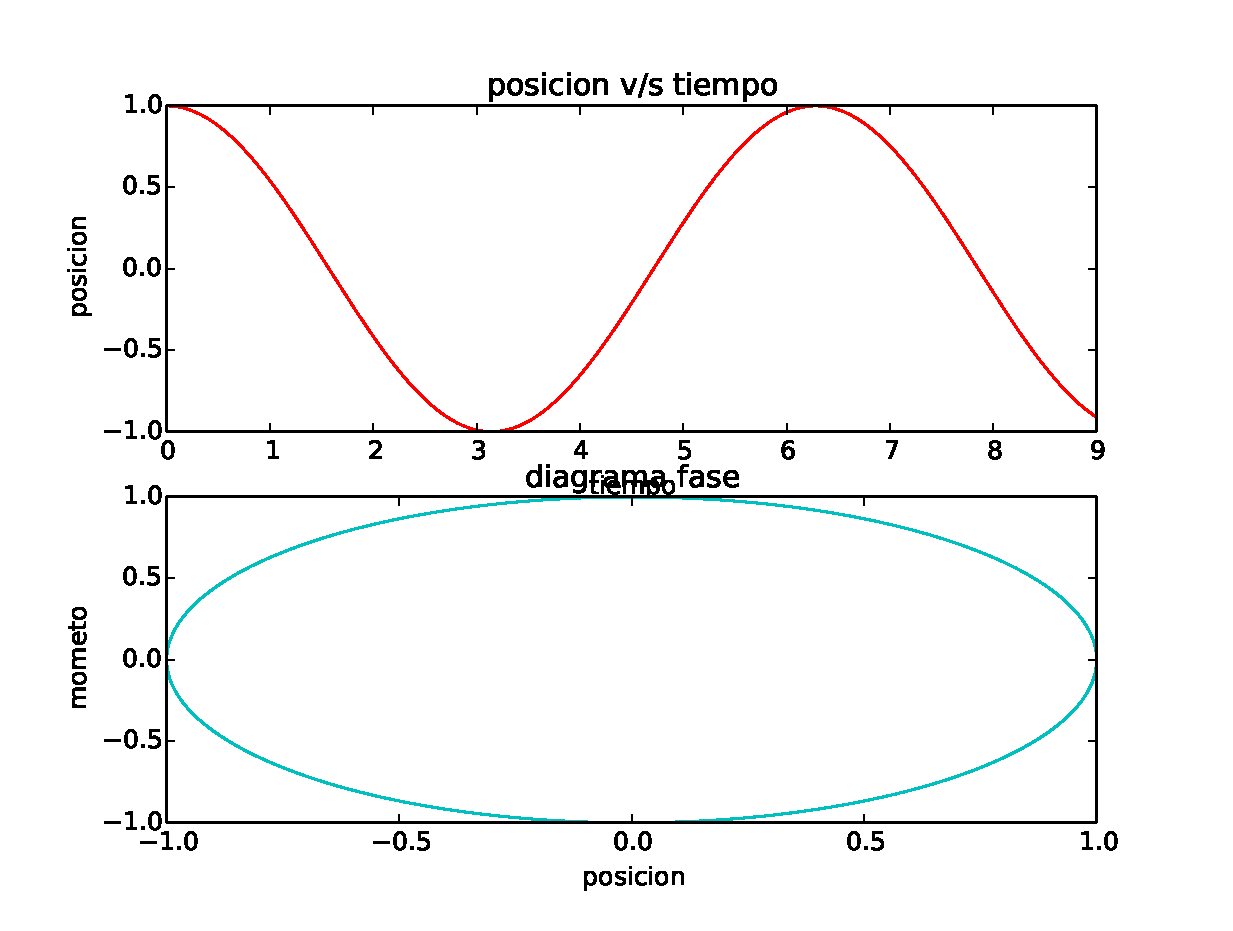
\includegraphics[scale=0.5]{Examen3_P1.eps}  
\end{figure}
\end{frame}
\begin{frame}
\frametitle{Cálculo del período. Modo 1.}
Sabemos de la tema anterior de integración que el período de un péndulo de longitud $L$ es $\tau = 4 \sqrt{\frac{L}{g}} h(\theta_{0})$, donde $g$ es la aceleración debida a la gravedad, $\theta_{0}$, representa la amplitud angular y 
\[ h(\theta_{0}) =  \int_{0}^{\frac{\pi}{2}} \dfrac{d\theta}{\sqrt{1 - \sin^{2} \left( \frac{\theta_{0}}{2}\right) \sin^{2} \theta}} \]
Lo que nos devuelve un valor del período de:
\[\tau=6.283207943236664, 6.975762127089018e-14\]
\end{frame}
\section{Problema 2}
\begin{frame}
\frametitle{Problema 2}
Un paracaidista de masa $m$ en caída libre vertical experimenta una fuerza de arrastre aerodinámica $F_{D} = c_{D} \dot{y}^{2}$, donde $y$ se mide hacia abajo a partir del comienzo de la caída. La EDO que describe la caída es
\[ \ddot{y} = g - \dfrac{c_{D}}{m} \dot{y}^{2}\]
Calcula el tiempo para una caída de 500 m, usa los valores de $g=9.80665 \mbox{ m/s}^{2}$, $c_{D}=0.2028 \mbox{ kg/m}$ y $m=80 \mbox{ kg}$.
\end{frame}
\begin{frame}[fragile]
\frametitle{Solución}
El conjunto de ecuaciones EDO-1 del problema:
\begin{lstlisting}
def F(x,y):
    F = np.zeros((2),dtype='float64')
    F[0] = y[1]
    F[1] = 9.80665-(0.2028/80.0)*(y[1]**2)
    return F
\end{lstlisting}
\end{frame}
\begin{frame}[fragile]
\frametitle{Solución gráfica}
\begin{figure}
	\centering
	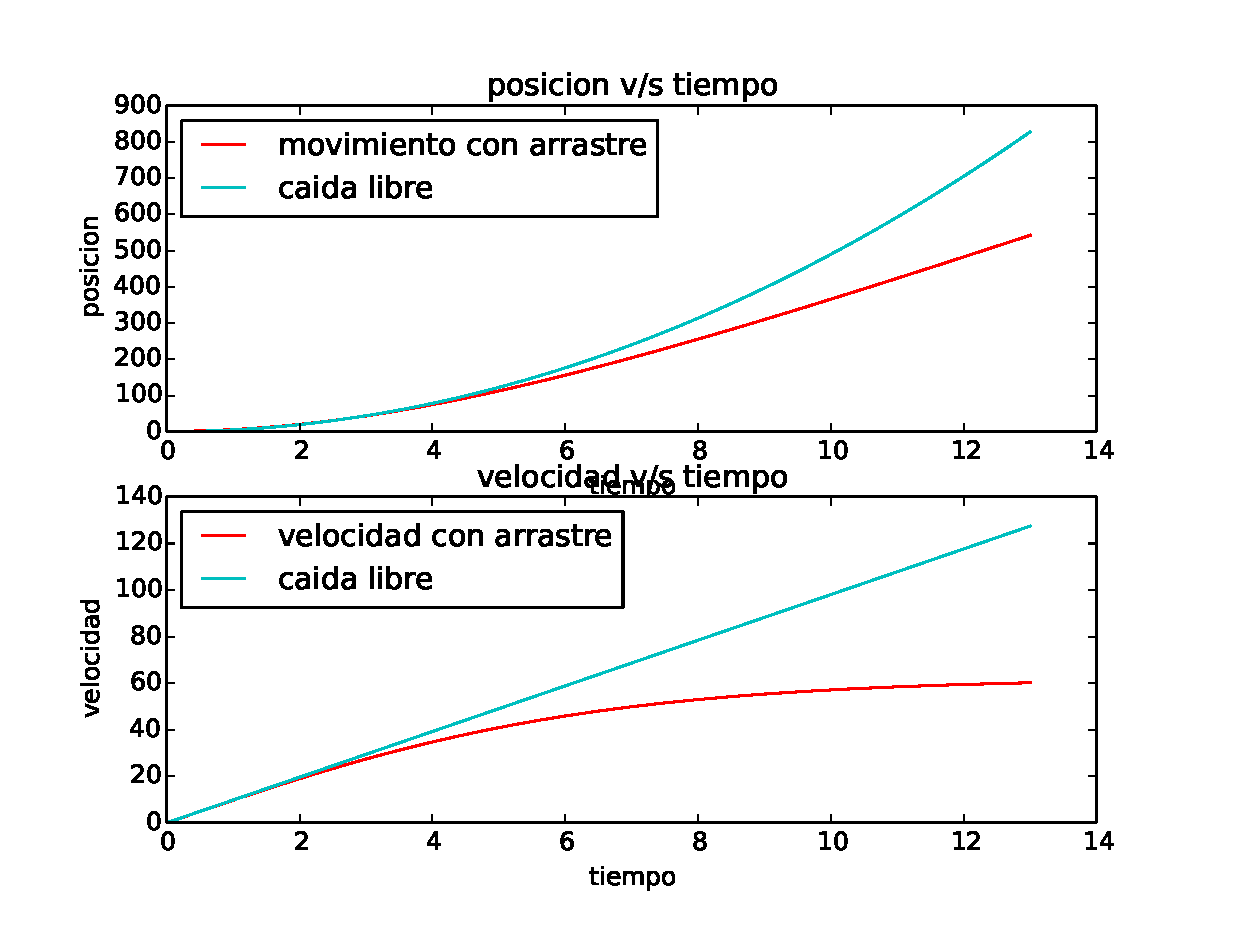
\includegraphics[scale=0.5]{Examen3_P2_01.eps}<1>  
	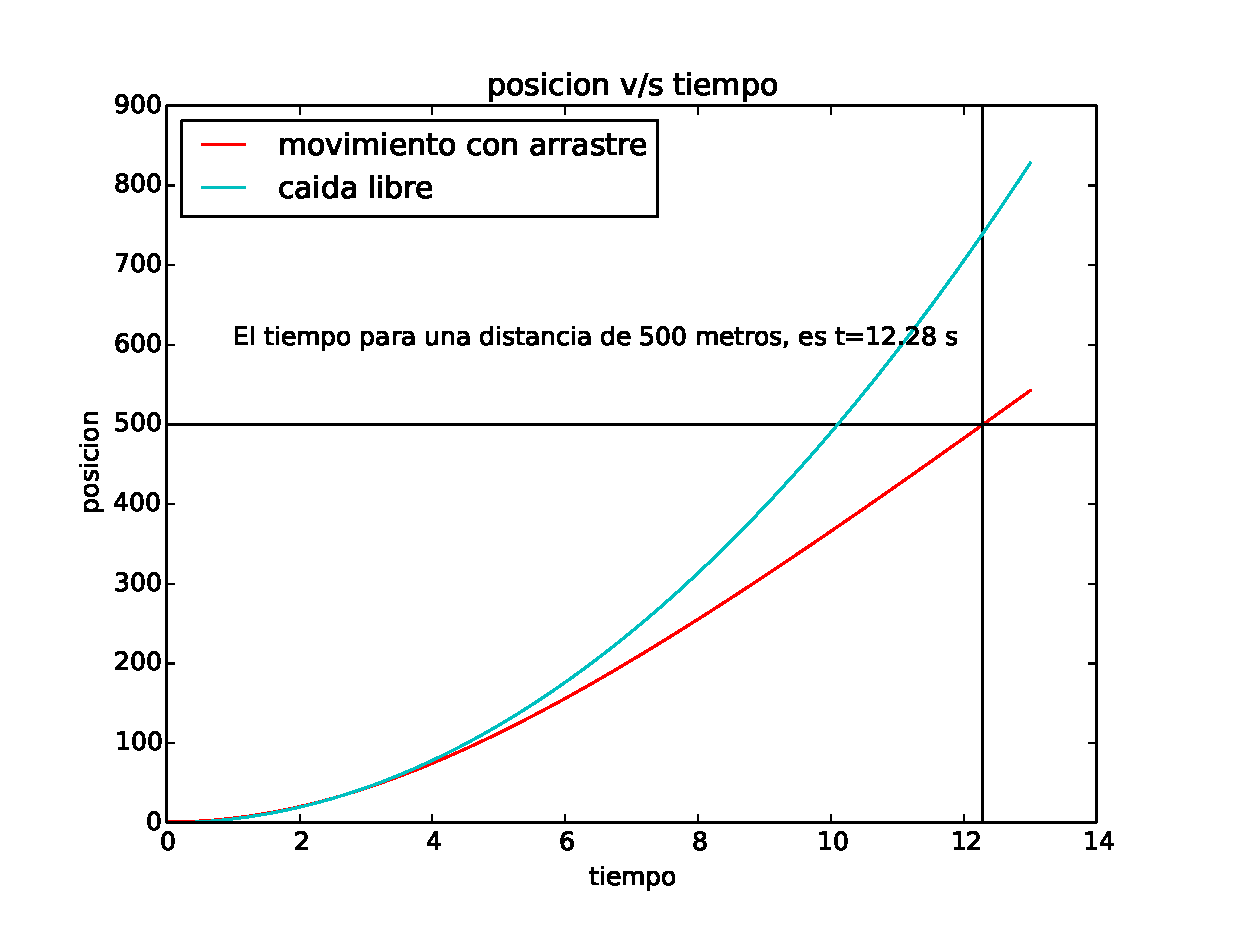
\includegraphics[scale=0.5]{Examen3_P2_02.eps}<2>
\end{figure}
\end{frame}
\section{Problema 3}
\begin{frame}
\frametitle{Problema 3}
Un sistema masa-resorte está en reposo hasta que se le aplica una fuerza $P(t)$, donde
\[ P(t) = \begin{cases}
10 t \mbox{ N para } t < 2 \mbox{ s} \\
20 \mbox{ N para } t \geq 2 \mbox{ s}
\end{cases} \]
\\
\begin{center}
\begin{tikzpicture}[font=\small]
	\tikzstyle{spring}=[thick,decorate,decoration={zigzag,pre length=0.3cm,post
	  length=0.3cm,segment length=6}]
	\draw (0,0) -- (5,0);
	\draw (0,0) -- (0,2);
	\draw [spring] (0,1) -- node [midway, above]{$k$}(2,1);
	\draw (2.5,0.1) circle (0.1);
	\draw (4,0.1) circle (0.1);
	\draw (2,0.2) rectangle node {$m$}(4.3,1.8);
	\draw [->,thick] (4.3,1) -- node [near end, above] {$P(t)$} (5.3,1);
\end{tikzpicture}
\end{center}
La EDO del movimiento resultante es
\[  \ddot{y} = \dfrac{P(t)}{m} - \dfrac{k}{m} y\]
Calcula el desplazamiento máximo de la masa. Usa $m=0.25$ kg y $k=75$ N/m.
\end{frame}
\begin{frame}[fragile]
\frametitle{Solución}
Como tenemos una fuerza que se aplica en dos momentos, hay que establecer las condiciones de la misma para los intervalos de tiempo que nos indica el problema.
\begin{lstlisting}
def F(x,y):
    F=np.zeros((2),dtype='float64')
    F[0]=y[1]
    F[1]=(1.0/0.25)*(10*x-75*y[0])
    return F

def G(x,y):
    G=np.zeros((2),dtype='float64')
    G[0]=y[1]
    G[1]=(1.0/0.25)*(20.0-75*y[0])
    return G
\end{lstlisting}
\end{frame}
\begin{frame}[fragile]
\frametitle{Gráfica de la solución}
\begin{figure}
	\centering
	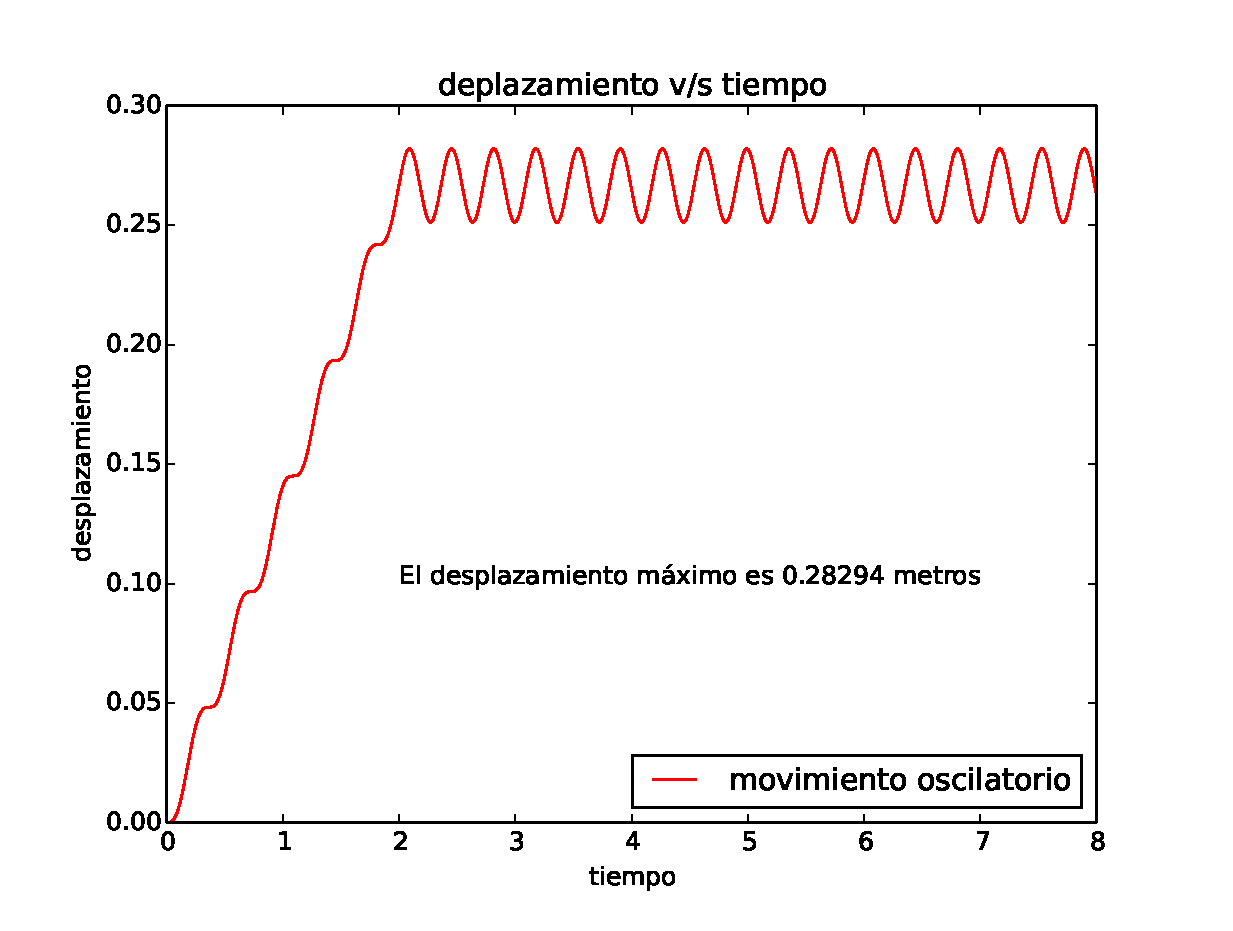
\includegraphics[scale=0.5]{Examen3_P3_01.eps}  
\end{figure}
\end{frame}
\section{Problema 4}
\begin{frame}
\frametitle{Problema 4}
Un flotador cónico se desliza libremente sobre una varilla vertical. Al tocar el flotador, éste pierde su posición de equilibrio, y presenta un movimiento oscilante que se describe por la ecuación diferencial:
\[ \ddot{y} = g (1 - a y^{3}) \]
donde $a=16 \mbox{ m}^{-3}$ (que están determinadas por la densidad y dimensiones del flotador) y $g=9.80665 \mbox{ m/s}^{2}$. 
\end{frame}
\begin{frame}[fragile]
\frametitle{El flotador cónico}
\begin{center}
\begin{tikzpicture}[font=\small]
	\draw [pattern = north east lines, draw =none] (0,0) rectangle (6,0.2);
	\draw [fill = blue!10, postaction={pattern = dots}, draw =none] (0,0.2) rectangle (6,3);
	\draw (0,0.2) -- (6,0.2);
	\draw (0,3) -- (6,3);
	\draw [fill = white](2.8,1.2) -- (3.2,1.2) -- (4.5,3.5) -- (1.5,3.5) -- cycle;
	\draw (2.9,0.2) rectangle (3.1,1.2);
	\draw [dashed](2.9,1.2) rectangle (3.1,3.5);
	\draw (2.9,3.5) rectangle (3.1,4.2);
	\draw (2.8,1.2) -- (1,1.2);
	\draw [<->] (1.2,1.2) -- node [midway, fill=white] {$y$} (1.2,3);
	\draw (0.5,4.2) node {Nivel del agua};
	\draw [->] (0.7,4) -- (0.9,3);
\end{tikzpicture}
\end{center}
Si el flotador se eleva a la posición $y=0.1$ m y se libera, determina el período y la amplitud de las oscilaciones.
\end{frame}
\begin{frame}[fragile]
\frametitle{Solución}
El sistema de EDO-1 que se obtiene para este problema es:
\begin{lstlisting}
def F(x,y):
    F=np.zeros((2),dtype='float64')
    F[0]=y[1]
    F[1]=9.80665*(1-16.0*y[0]**3)
    return F
\end{lstlisting}
\end{frame}
\begin{frame}[fragile]
\frametitle{Solución gráfica}
\begin{figure}
	\centering
	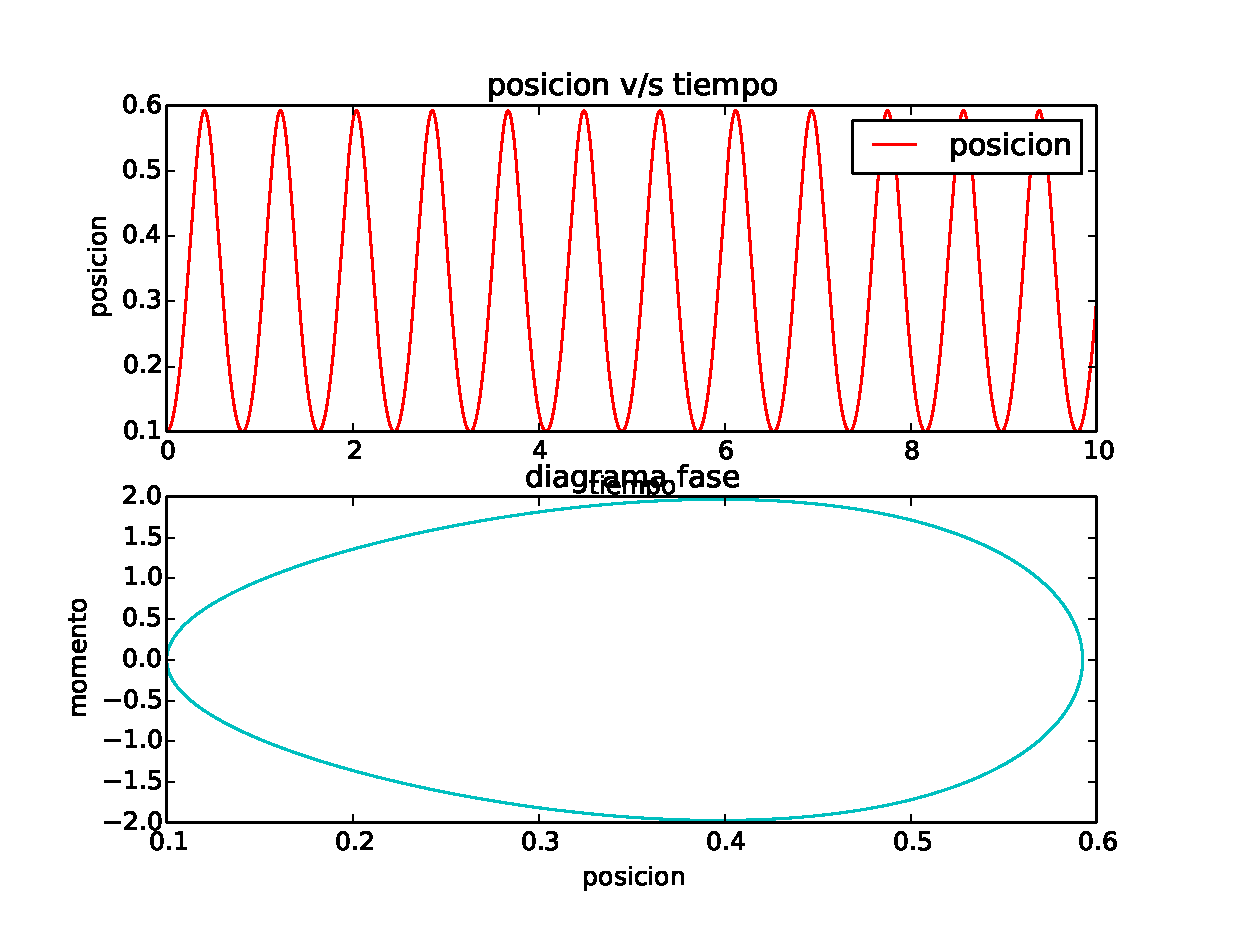
\includegraphics[scale=0.5]{Examen3_P4_01.eps}<1>  
	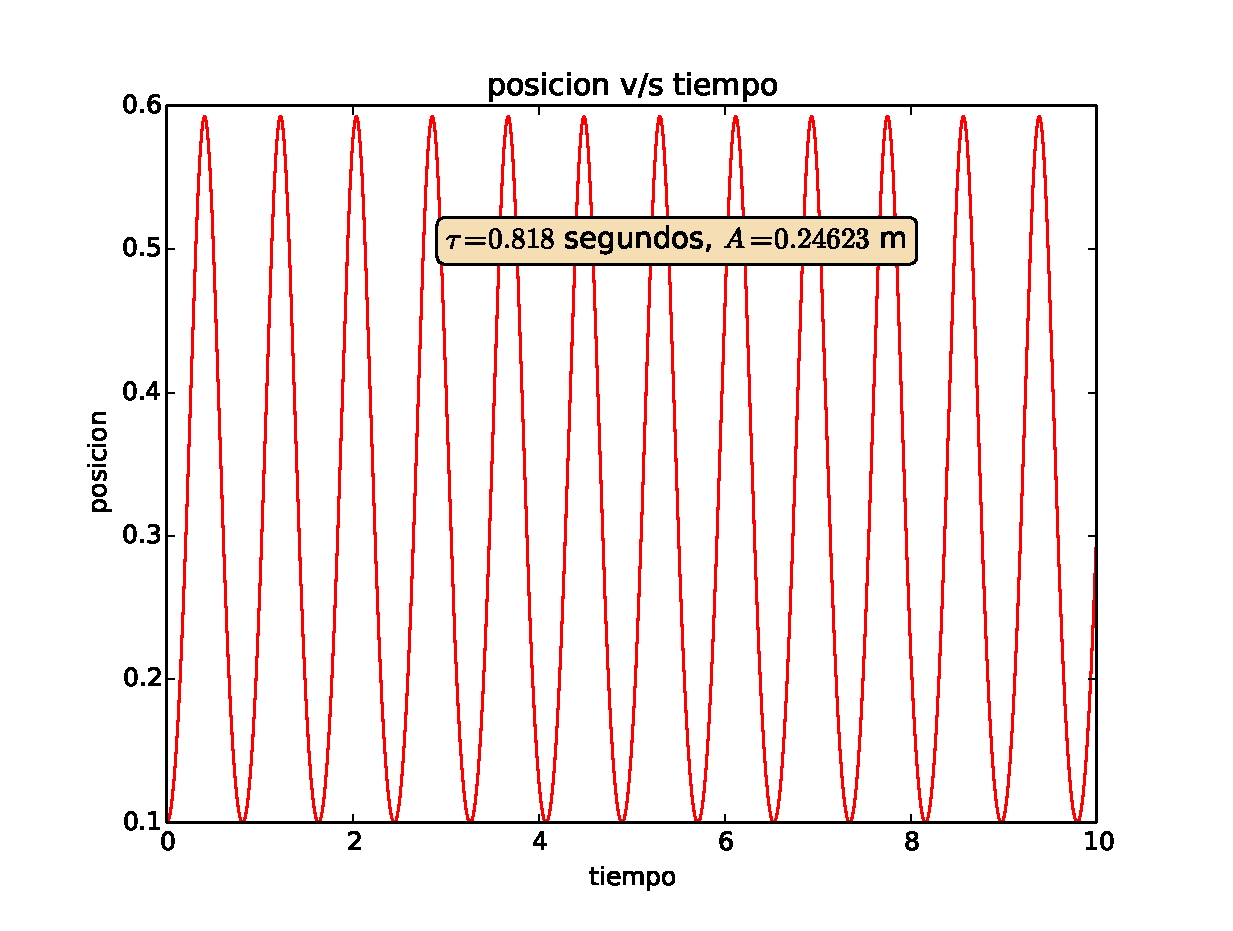
\includegraphics[scale=0.5]{Examen3_P4_02.eps}<2>
\end{figure}
\end{frame}
\section{Problema 5}
\begin{frame}
\frametitle{Problema 5}
Un péndulo está suspendido en un collar deslizante. El sistema está en reposo, posteriormente se aplica al collar un movimiento oscilante $y(t) = Y \sin \omega t$, en $t=0$. La ecuación diferencial que describe el movimiento del péndulo es
\[ \ddot{\theta} = - \dfrac{g}{L} \sin \theta + \dfrac{\omega^{2}}{L} Y \cos \theta \sin \omega t\]
\begin{center}
\begin{tikzpicture}[font=\small]
	\draw (-0.1,-0.2) [pattern = north east lines] rectangle (0.1,0.4);
	\draw (4.9,-0.2) [pattern = north east lines] rectangle (5.1,0.4);
	\draw (0.1,0.0) rectangle (4.9,0.2);
	\draw (2.1,-0.1) [fill=white] rectangle (2.9,0.3);
	\draw [dashed] (2.5,-1.5) -- (2.5,0.7);
	\draw [->, thick] (2.5,0.6) -- node [right=0.6cm] {$y(t)$} (3.5,0.6);
	\draw [thick] (2.5,0.1) -- node [near end, above=0.5cm]{$L$}(3.51,-2.);
	\draw (3.6,-2.2) circle (0.2) node [right=0.2cm] {$m$};
	\draw (2.5,-0.45) arc (270:290:7mm) node [below=0.15cm]{$\theta$};
\end{tikzpicture}
\end{center}
\end{frame}
\begin{frame}
Grafica $\theta$ contra $t$ en el intervalo de $t=0$ a $t=10$ segundos, así mismo, determina el desplazamiento mayor de $\theta$ durante éste período. Usa $g=9.80665$ m/$s^{2}$, $L=1.0$ m, $Y=0.25$ m y $\omega = 2.5$ rad/s.
\end{frame}
\begin{frame}[fragile]
\frametitle{Solución}
El sistema de EDO-1 necesario para resolver el problema es:
\begin{lstlisting}
def F(x,y):
    F=np.zeros((2),dtype='float64')
    F[0]=y[1]
    F[1]=(-9.80665/1.0)*np.sin(y[0])+((2.5**2)*0.25)*(np.cos(y[0]))*np.sin(2.5*x)
    return F
\end{lstlisting}
\end{frame}
\begin{frame}[fragile]
\frametitle{Solución gráfica}
\begin{figure}
	\centering
	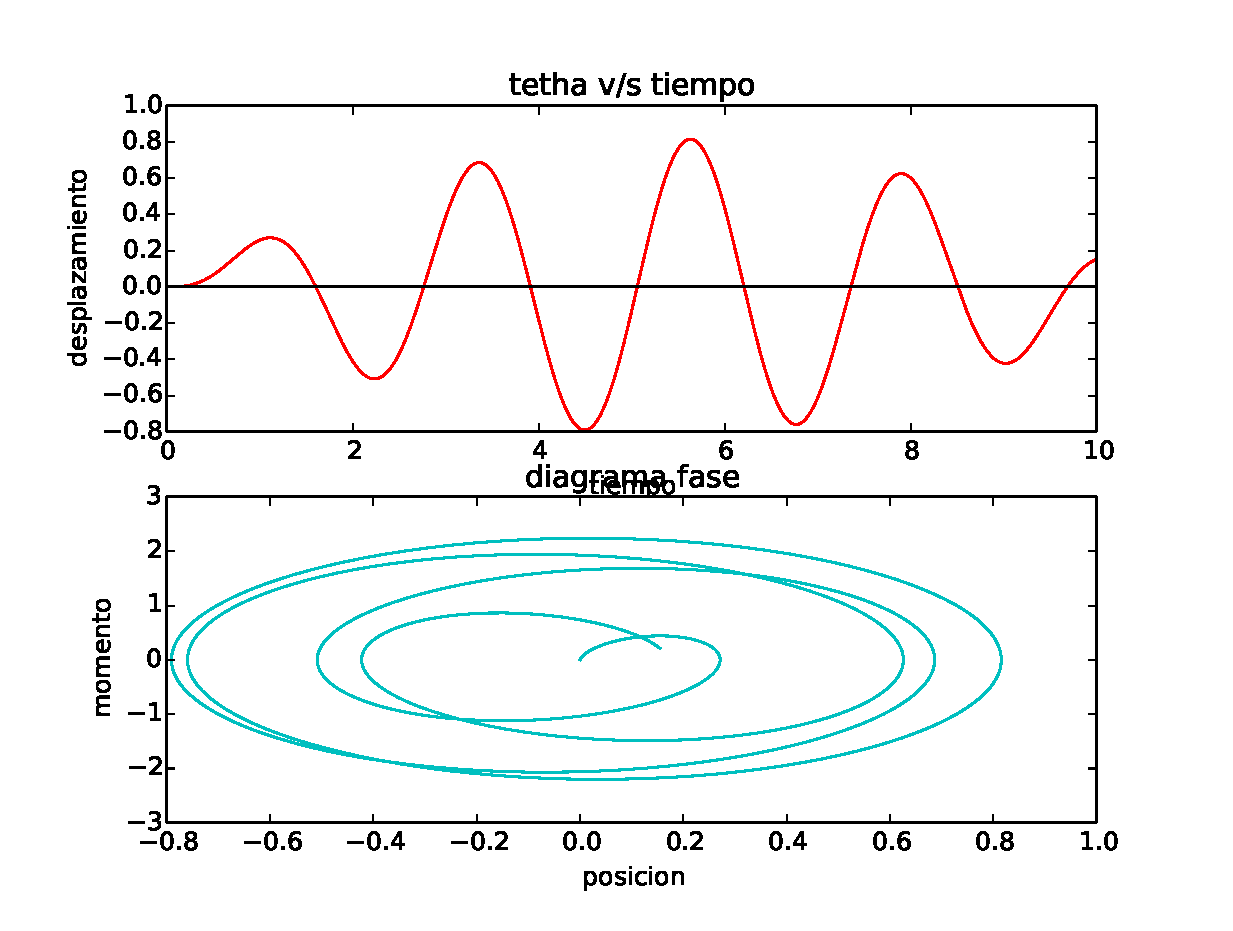
\includegraphics[scale=0.5]{Examen3_P5_01.eps}<1>  
	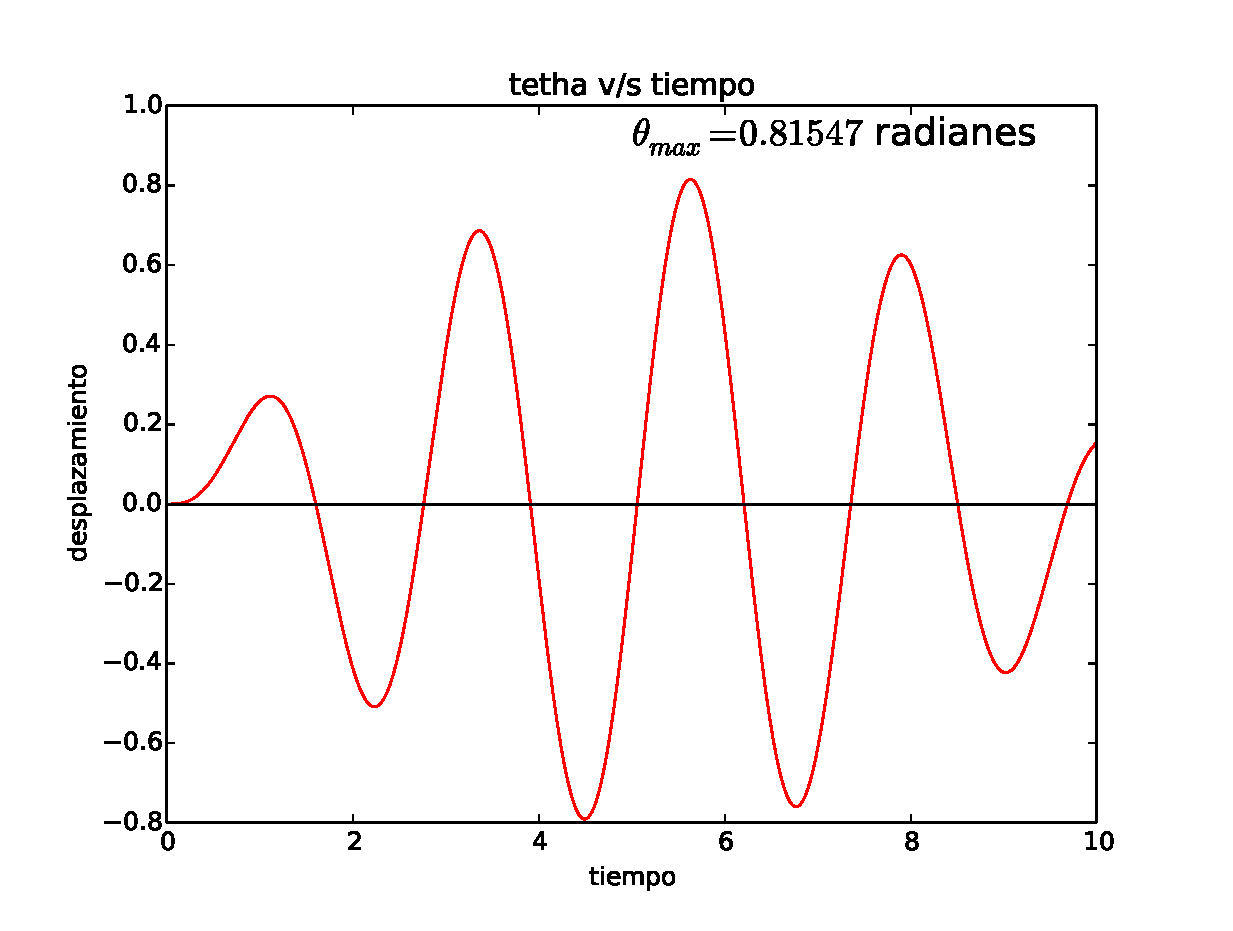
\includegraphics[scale=0.5]{Examen3_P5_02.eps}<2>
\end{figure}
\end{frame}
\section{Problema 6}
\begin{frame}
\frametitle{Problema 6}
Tenemos un sistema que consiste en un masa que se desliza sobre una barra guíaa que está en reposo, la masa se ubica en $r=0.75$ m. Al tiempo $t=0$ se enciende un motor que proporiona un movimiento dado por la expresión $\theta(t) = (\pi/12) \cos \pi t$ sobre la barra. La EDO que describe el movimiento resultante de la masa deslizante es:
\[ \ddot{r} = \left( \dfrac{\pi^{2}}{12}\right)^{2}  r \sin^{2} \pi t - g \sin \left( \dfrac{\pi}{12} \cos \pi t \right) \]
\end{frame}
\begin{frame}[fragile]
\begin{center}
\begin{tikzpicture}[font=\small]
	\draw (0,0) [pattern = north east lines] rectangle (2,0.2);
	\draw (0.2,0.2) -- (0.55,1.2);
	\draw (1.8,0.2) -- (1.45,1.2);
	\draw (0.9,0.9) [rotate around={15:(1,1)}]rectangle (6,1.15);
	\draw (1,1) [fill=white] circle (0.5);
	\draw (1,1) circle (0.1);
	\draw (4,0.7) [fill=white, rotate around={15:(1,1)}]rectangle (4.5,1.4);
	\draw (2,1) -- (4,1);
	\draw (3.4,1) arc (0:25:12mm);
	\draw (3.8,1.3) node {$\theta(t)$};
	\draw (0.8,1.6) [rotate around={15:(0.8,1.6)}] -- (0.8,3);
	\draw (4,2.3) [rotate around={15:(4,2.3)}] -- (4,3);
	\draw (5.75,2.5) [rotate around={15:(5.75,2.5)}] -- (5.75,4.3);
	\draw [<->,rotate around={15:(0.7,2)}] (0.7,2)  -- node [rotate=15,midway, fill=white]{$r$}(4,2);
	\draw [<->,rotate around={15:(0.5,2.8)}] (0.5,2.8)  -- node [rotate=15,midway, fill=white]{$2 \mbox{ m}$}(5.5,2.8);
	\end{tikzpicture}
\end{center}
Calcula el tiempo para el cual, la masa deslizante alcanza el extremo final de la barra guía (la punta de la barra). Usa el valor de $g=9.80665 \mbox{ m/s}^{2}$.
\end{frame}
\begin{frame}[fragile]
\frametitle{Solución}
Establecemos el conjunto de EDO-1
\begin{lstlisting}
def F(x,y):
    F=np.zeros((2),dtype='float64')
    F[0]=y[1]
    F[1]=(((np.pi**2)/12.0)**2)*y[0]*((np.sin((np.pi)*x))**2) \
         -9.80665*(np.sin((np.pi/12.0)*(np.cos(x*np.pi))))
    return F
\end{lstlisting}
\end{frame}
\begin{frame}[fragile]
\frametitle{Solución gráfica}
\begin{figure}
	\centering
	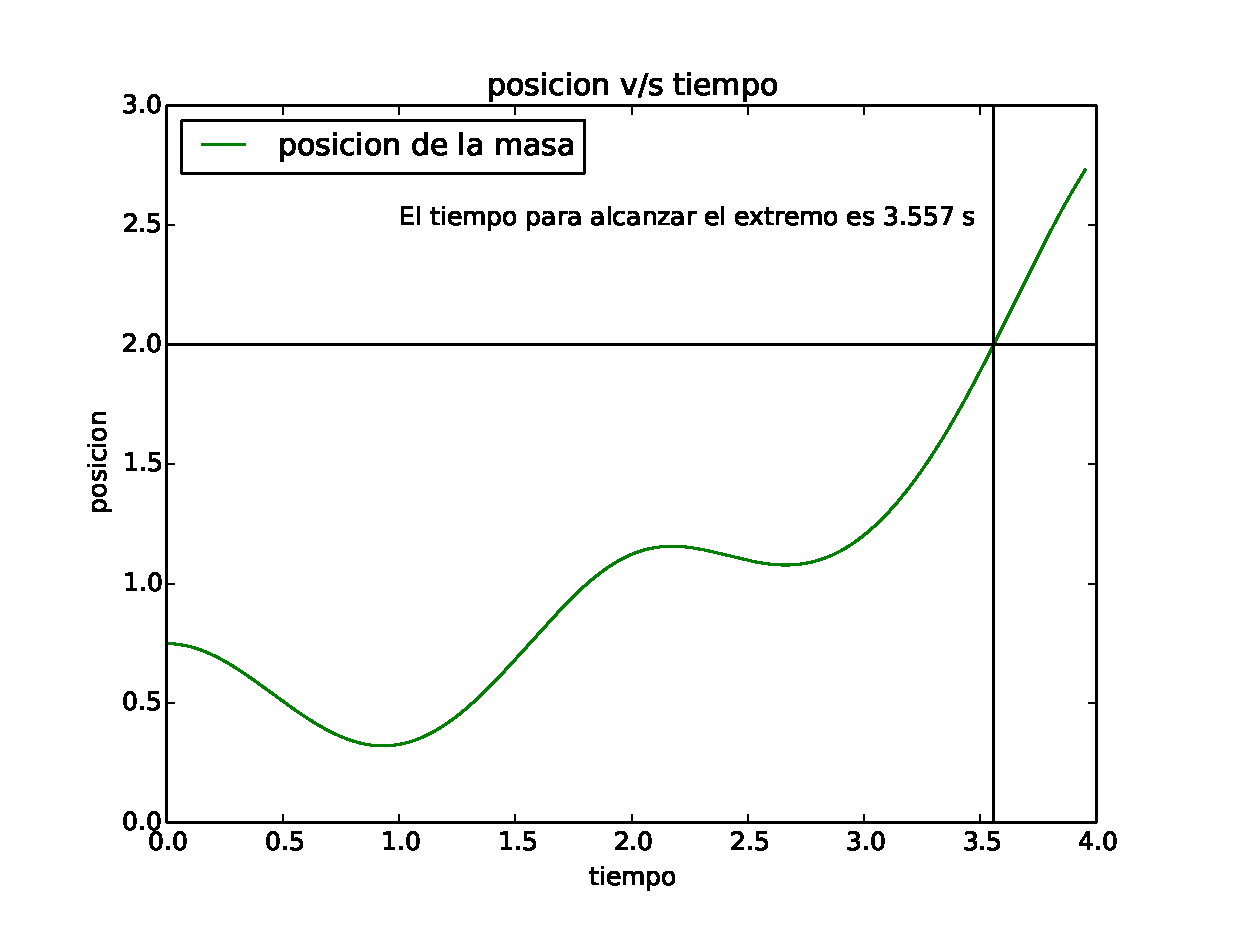
\includegraphics[scale=0.5]{Examen3_P6_01.eps}
\end{figure}
\end{frame}
\section{Problema 7}
\begin{frame}[fragile]
\frametitle{Problema 7}
Una bala de masa $m=0.25$ kg se lanza con una velocidad $v_{0}= 50$ m/s en la dirección que se indica en la figura. Si la fuerza aerodinámica de arrastre sobre la bala es $F_{D}= C_{D} v^{3/2}$, las ecuaciones diferenciales que describen el movimiento son:
\[\ddot{x} = - \dfrac{C_{D}}{m} \dot{x} v^{1/2} \hspace{2cm} \ddot{y}= - \dfrac{C_{D}}{m} \dot{y} v^{1/2} - g\]
donde $v=\sqrt{\dot{x}^{2} + \dot{y}^{2}}$, $C_{D} = 0.03 \mbox{ kg/(ms)}^{1/2}$ y $g=9.80665 \mbox{m/s}^{2}$.
\end{frame}
\begin{frame}[fragile]
Calcular el tiempo de vuelo y el alcance $R$
\begin{center}
\begin{tikzpicture}[font=\small]
	\draw (0,0) [pattern = north east lines, draw = none] rectangle (6,0.5);
	\draw (0,0.5) -- node [midway, above] {$R$} (6.3,0.5);
	\draw (1,0.5) -- node [near end, left] {$y$} (1,3);
	\draw [fill=white] (1,0.5) circle (0.1);
	\draw (0.6,0.8) node {$m$};
	\draw [->, rotate around={30:(1,0.5)}, thick] (1,0.5) -- node [near end, above] {$v_{0}$} (3,0.5);
	\draw (2,0.5) arc (0:30:10mm);
	\draw (2.5,0.8) node {$30^{\circ}$};
	\draw (1,0.5) .. controls (3.8,2.2) and (4.6,2.4) .. (5.5,0.5);
%		  (4,2) .. controls (3.9,1.9).. and (4.1,2.1)..(5.5,0.5);
%		  (3.3,1.4) ..controls (4,1.5) and (4.2,1.3) .. (5.5,0.2);%.. controls (3.8,0.3) and (3.5,0.2) .. (5.5,0);
\end{tikzpicture}
\end{center}
\end{frame}
\begin{frame}[fragile]
\frametitle{Solución}
Establecemos el conjunto de EDO-1
\begin{lstlisting}
def F(x,y):
    F=np.zeros((4),dtype='float64')
    F[0]=y[1]
    F[1]=-(0.03/0.25)*y[1]*(np.sqrt(y[1]**2+y[3]**2))
    F[2]=y[3]
    F[3]=-(0.03/0.25)*y[3]*(np.sqrt(y[1]**2+y[3]**2))-9.80665
    return F
\end{lstlisting}
\end{frame}
\begin{frame}[fragile]
\frametitle{Solución gráfica}
\begin{figure}
	\centering
	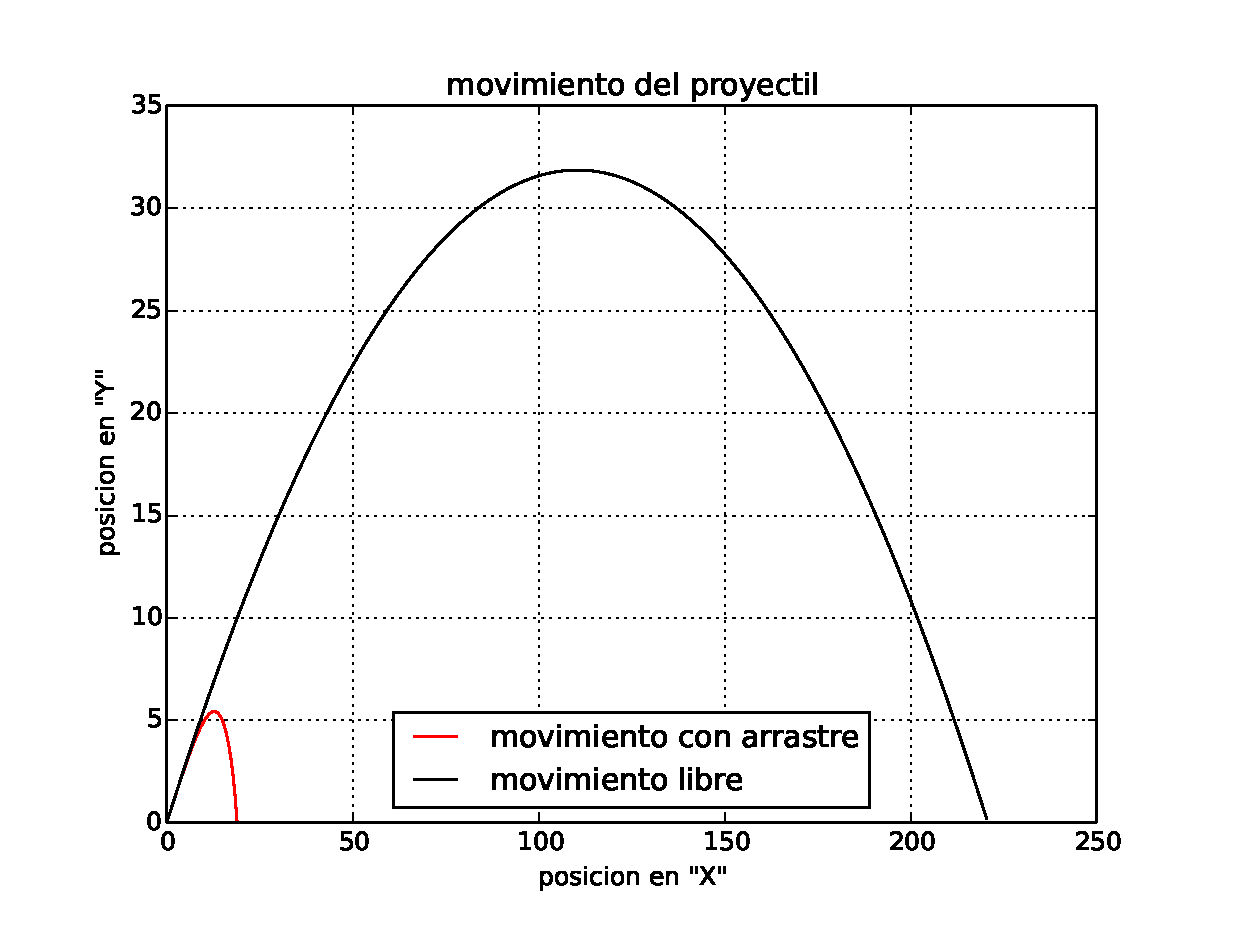
\includegraphics[scale=0.5]{Examen3_P7_01.eps}<1>
	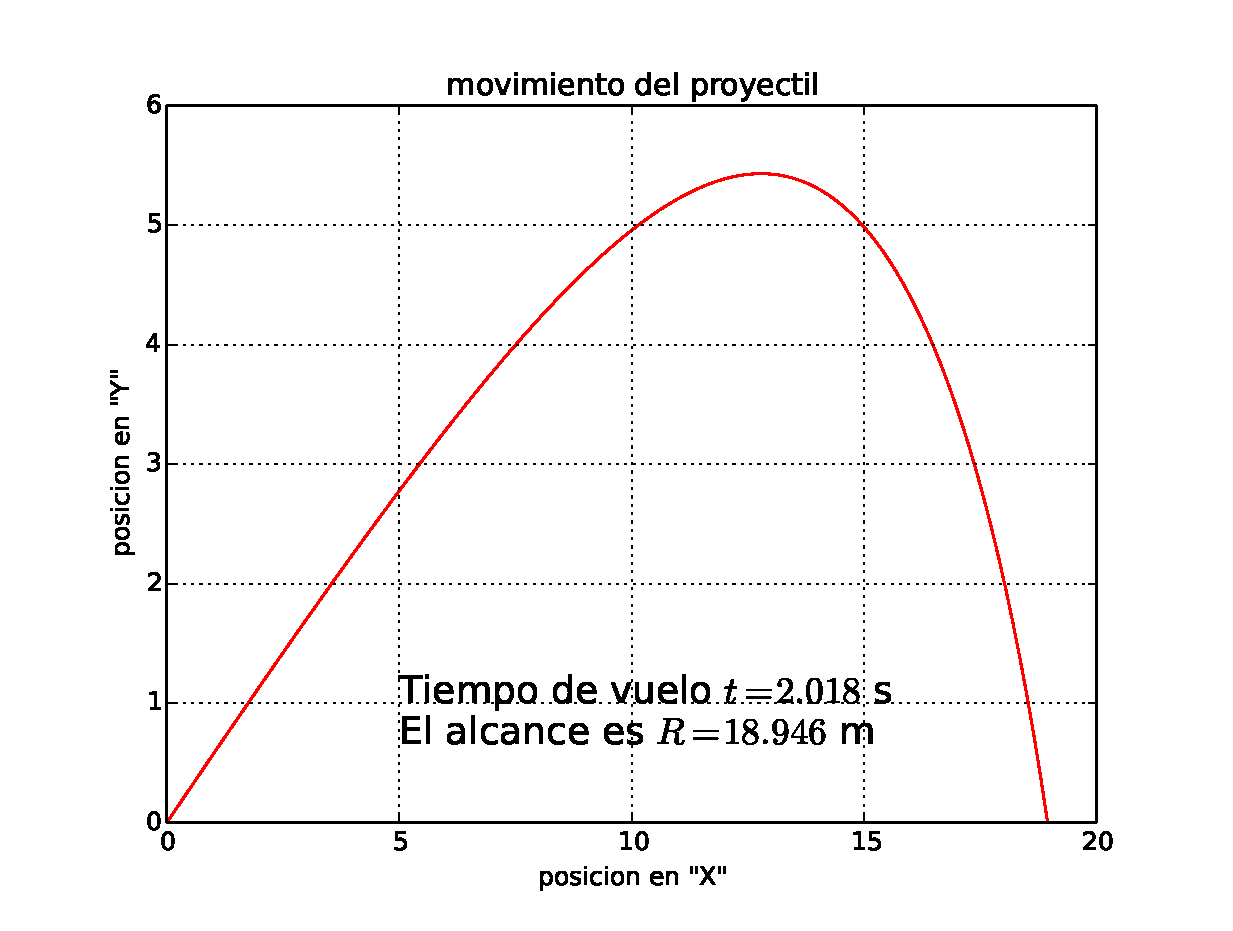
\includegraphics[scale=0.5]{Examen3_P7_02.eps}<2>
\end{figure}
\end{frame}
\section{Problema 8}
\begin{frame}
\frametitle{Problema 8}
La solución al problema
\[ y'' + \dfrac{1}{x} y' + y \hspace{1.5cm} y(0)=1 \hspace{1cm} y'(0)=0\]
es la función de Bessel $J_{0}(x)$. Integra numéricamente para calcular $J_{0}(5)$ y compara el resultado con $-0.17760$, que es el valor que se obtiene de tablas matemáticas. Tip: para evitar la singularidad en $x=0$, inicia la integración en $x=10^{-12}$.
\end{frame}
\begin{frame}[fragile]
\frametitle{Solución}
Establecemos el conjunto de EDO-1
\begin{lstlisting}
def F(x,y):
    F=np.zeros((2),dtype='float64')
    F[0]=y[1]
    F[1]=-(1.0/x)*y[1]-y[0]
    return F
\end{lstlisting}
\end{frame}
\begin{frame}
\frametitle{Solución gráfica}
\begin{figure}
	\centering
	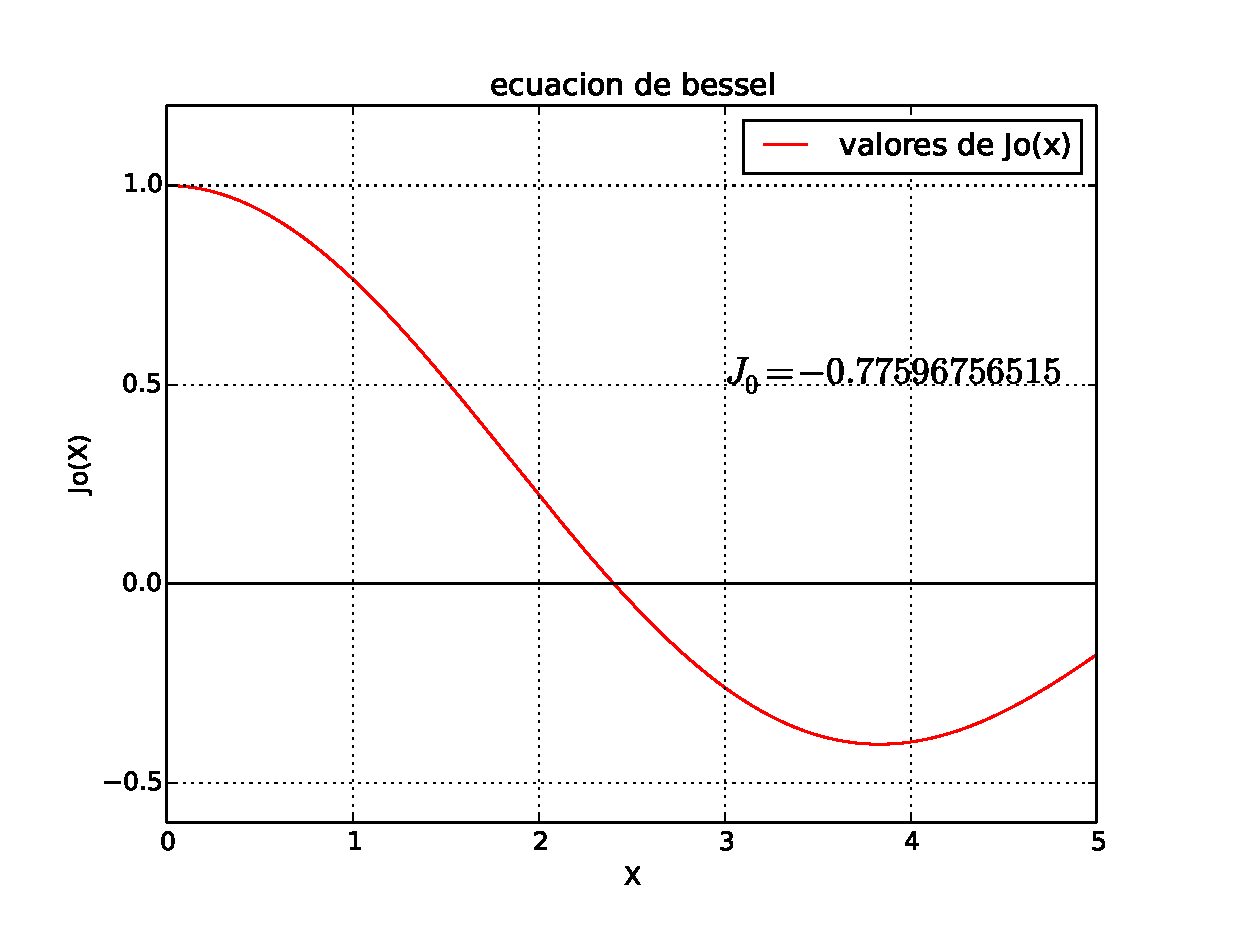
\includegraphics[scale=0.5]{Examen3_P8_01.eps}
\end{figure}
\end{frame}
\end{document}